% =====================================================================
%  第三章  页表系统改造
% =====================================================================
\chapter{页表系统改造}

\section{设计目标与页表布局}
页表系统是本次改造的根基。原系统用一张相对虚实地址映射表充当所有进程共用的
"物理页表"，进程切换时需重写页表项；本设计的目标是让\textbf{每个进程拥有独立的
页目录}，进程切换时通过更换 \texttt{CR3} 寄存器即可完成地址空间切换，从而既支持
进程间地址空间隔离，也减少切换开销。

改造后的虚实地址空间分布沿用 UNIX V6++ 的既有设计（对应课设 PPT slide 4\,–\,6）。
物理内存自低地址起依次为：保留区（0\,–\,1M）、
内核（1M 起）、内核堆对象区（1.5M 起）、页表区（2M 起）、用户区（4M 起）。其中
页表区的物理布局具有关键意义：

\begin{itemize}
  \item \texttt{0x200000}（即 0x200 号页框）：全局\textbf{页目录}（Page Directory），
        由 \texttt{Machine::PAGE\_DIRECTORY\_BASE\_ADDRESS} 标识；
  \item \texttt{0x201000}（0x201 号页框）：\textbf{核心页表}（Page Table 768\#），
        映射内核空间，所有进程共享；
  \item \texttt{0x202000}（0x202 号页框）：\textbf{0\# 用户页表}（Page Table 0\#），
        全局共享；
  \item \texttt{0x203000} 起（0x203 号及以后页框）：各进程\textbf{私有 1\# 用户页表}
        （Page Table 1\#），进程创建时动态分配。
\end{itemize}

\begin{figure}[H]
  \centering
  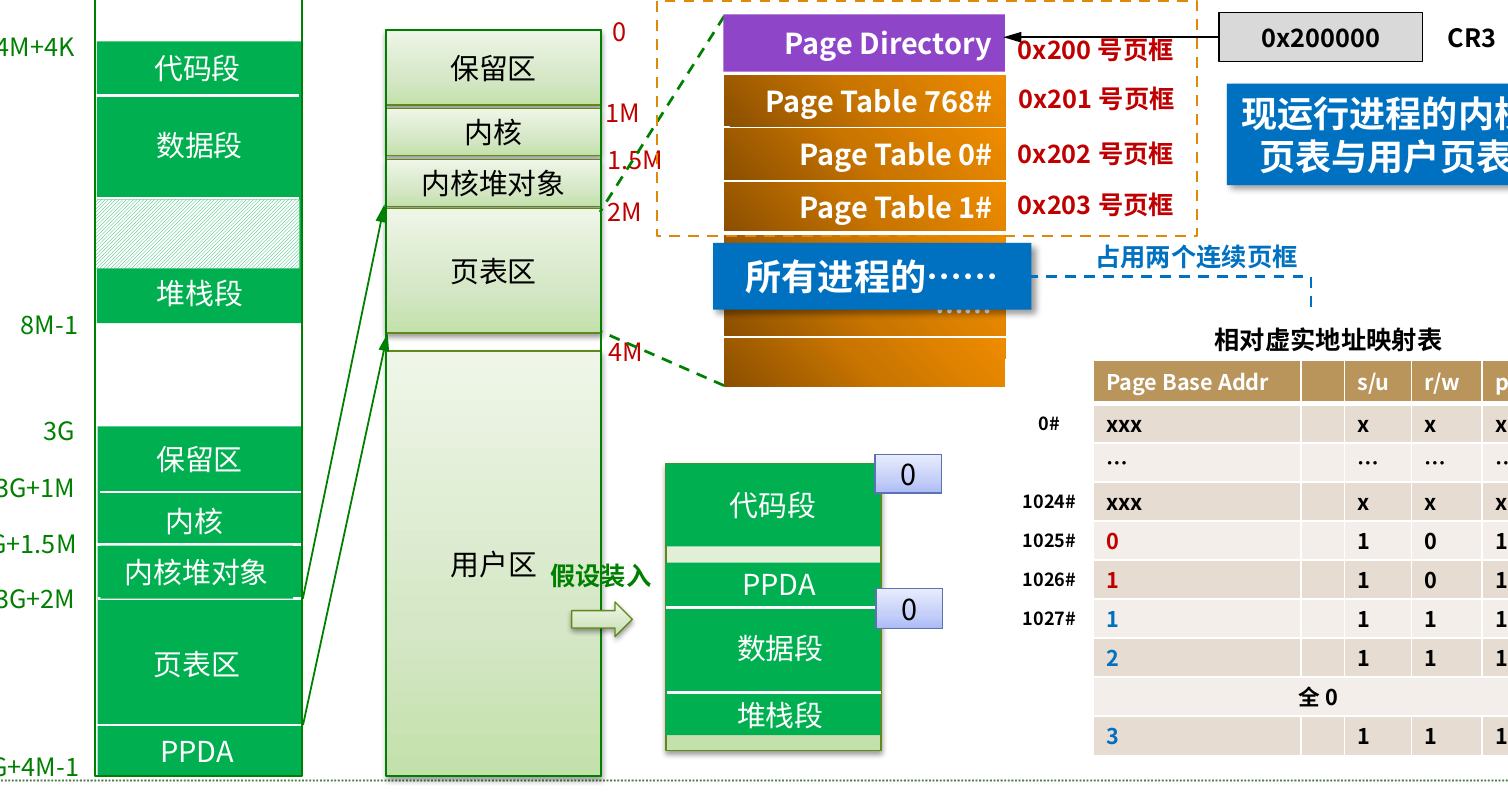
\includegraphics[width=0.9\textwidth]{figures/fig_pt_struct.png}
  \caption{页目录、页表与页框的构成关系（图源：课程设计 PPT slide 6）}
  \label{fig:pt-struct}
\end{figure}

在 80386 的两级页表机制下，一个页目录含 1024 个页目录项（PDE），每项指向一张页表；
一张页表含 1024 个页表项（PTE），每项映射一个 4KB 页框，故一张页表覆盖 4MB 虚拟
空间（\texttt{PageTable::SIZE\_PER\_PAGETABLE\_MAP = 0x400000}）。本设计中内核空间
固定从 \texttt{0xC0000000}（3G）起的 4MB，恰好对应页目录的第 768 项（
\texttt{0xC0000000 / 0x400000 = 768}）；用户空间从 0 起的 8MB 则由 0\# 与 1\# 两张
用户页表共同覆盖。

\section{内核页表与共享用户页表初始化}
并非所有页表都需要随进程切换。核心页表与 0\# 用户页表的内容对所有进程都相同，
因此被设计为\textbf{全局共享}，只在系统初始化时建立一次。\texttt{Machine} 类为此
新增了两个初始化接口（\texttt{Machine.h}，标注 NOTE 3）：

\begin{lstlisting}[caption={核心页表与共享用户页表的初始化接口},label={lst:machine-init}]
// 对应源码 include/Machine.h
void InitKernelPageTable();   // 初始化所有进程共享的核心页表(768#)
void InitZeroUserPageTable(); // 初始化所有进程共享的 0# 用户页表
\end{lstlisting}

其中，核心页表（768\#）把内核空间 \texttt{0xC0000000}\,–\,\texttt{0xC0400000} 恒等
映射到物理内存 \texttt{0x00000000}\,–\,\texttt{0x00400000}（即内核实际加载位置），
使得内核代码无论哪个进程运行都能被正确访问；0\# 用户页表则作为用户空间低 4MB 的
"共享窗口"，在 \texttt{exec} 构造参数栈时被临时借用（详见第五章）。

对于系统中的第一个进程——0\# 进程，其页目录在
\texttt{ProcessManager::SetupProcessZero()} 中被固定设置在页表区起始的物理页框上：

\begin{lstlisting}[caption={0\# 进程页目录的设置},label={lst:setup-zero}]
// 对应源码 proc/ProcessManager.cpp :: SetupProcessZero
pProcZero->pPageDirectory =
    (PageDirectory *)(Machine::PAGE_DIRECTORY_BASE_ADDRESS
                      + Machine::KERNEL_SPACE_START_ADDRESS);
// 物理地址 0x200000 + 虚地址偏移 0xC0000000 => 内核可访问的逻辑地址
\end{lstlisting}

注意此处把物理地址 \texttt{0x200000} 加上内核空间起始虚地址 \texttt{0xC0000000}，
得到内核视角下访问该页目录的逻辑地址——这正是核心页表恒等映射的用途。

\section{进程私有页目录与私有用户页表}
除共享部分外，每个进程还需要属于自己的页目录与一张私有 1\# 用户页表。为此，
\texttt{Process} 类新增了指向本进程页目录的指针及一个将其换算为物理地址的接口
（\texttt{include/Process.h}，标注 NOTE 3）：

\begin{lstlisting}[caption={Process 类新增的页目录成员},label={lst:proc-pdir}]
public:
    PageDirectory *pPageDirectory;          // 指向本进程页目录的逻辑地址
    unsigned long GetPageDirectoryPhyAddr();// 换算为物理地址, 供写入 CR3
\end{lstlisting}

\texttt{GetPageDirectoryPhyAddr()} 的实现十分直接——由于 \texttt{pPageDirectory}
保存的是内核空间逻辑地址，减去内核空间起始地址 \texttt{0xC0000000} 即得物理地址。

进程创建时，\texttt{ProcessManager} 提供两个辅助函数来建立私有页目录：
\texttt{AllocPageDirectory()} 从内核页框池分配一页作为页目录；
\texttt{InitProcPageDirectory()} 则把三类页表项填入新页目录——共享的 0\# 用户页表、
核心页表，以及本进程私有的 1\# 用户页表：

\begin{lstlisting}[caption={进程私有页目录的初始化},label={lst:init-pdir}]
// 对应源码 proc/ProcessManager.cpp :: InitProcPageDirectory
void ProcessManager::InitProcPageDirectory(Process *proc, PageTable *privateUsrPageTable)
{
    PageDirectory *pPageDirectory = proc->pPageDirectory;
    // (1) 共享的 0# 用户页表
    pPageDirectory->m_Entrys[0].m_UserSupervisor   = 1;
    pPageDirectory->m_Entrys[0].m_Present           = 1;
    pPageDirectory->m_Entrys[0].m_ReadWriter        = 1;
    pPageDirectory->m_Entrys[0].m_PageTableBaseAddress = Machine::USER_PAGE_TABLE_BASE_ADDRESS >> 12;
    // (2) 核心页表 (页目录第 768 项)
    unsigned int kPageTableIdx = Machine::KERNEL_SPACE_START_ADDRESS / PageTable::SIZE_PER_PAGETABLE_MAP;
    pPageDirectory->m_Entrys[kPageTableIdx].m_UserSupervisor = 0;   // 内核态
    pPageDirectory->m_Entrys[kPageTableIdx].m_Present          = 1;
    pPageDirectory->m_Entrys[kPageTableIdx].m_ReadWriter       = 1;
    pPageDirectory->m_Entrys[kPageTableIdx].m_PageTableBaseAddress = Machine::KERNEL_PAGE_TABLE_BASE_ADDRESS >> 12;
    // (3) 私有 1# 用户页表 (本进程独有)
    unsigned long phyFrame = ((unsigned long)privateUsrPageTable - Machine::KERNEL_SPACE_START_ADDRESS) >> 12;
    pPageDirectory->m_Entrys[1].m_PageTableBaseAddress = phyFrame;
    pPageDirectory->m_Entrys[1].m_UserSupervisor = 1;
    pPageDirectory->m_Entrys[1].m_Present          = 1;
    pPageDirectory->m_Entrys[1].m_ReadWriter       = 1;
}
\end{lstlisting}

\begin{figure}[H]
  \centering
  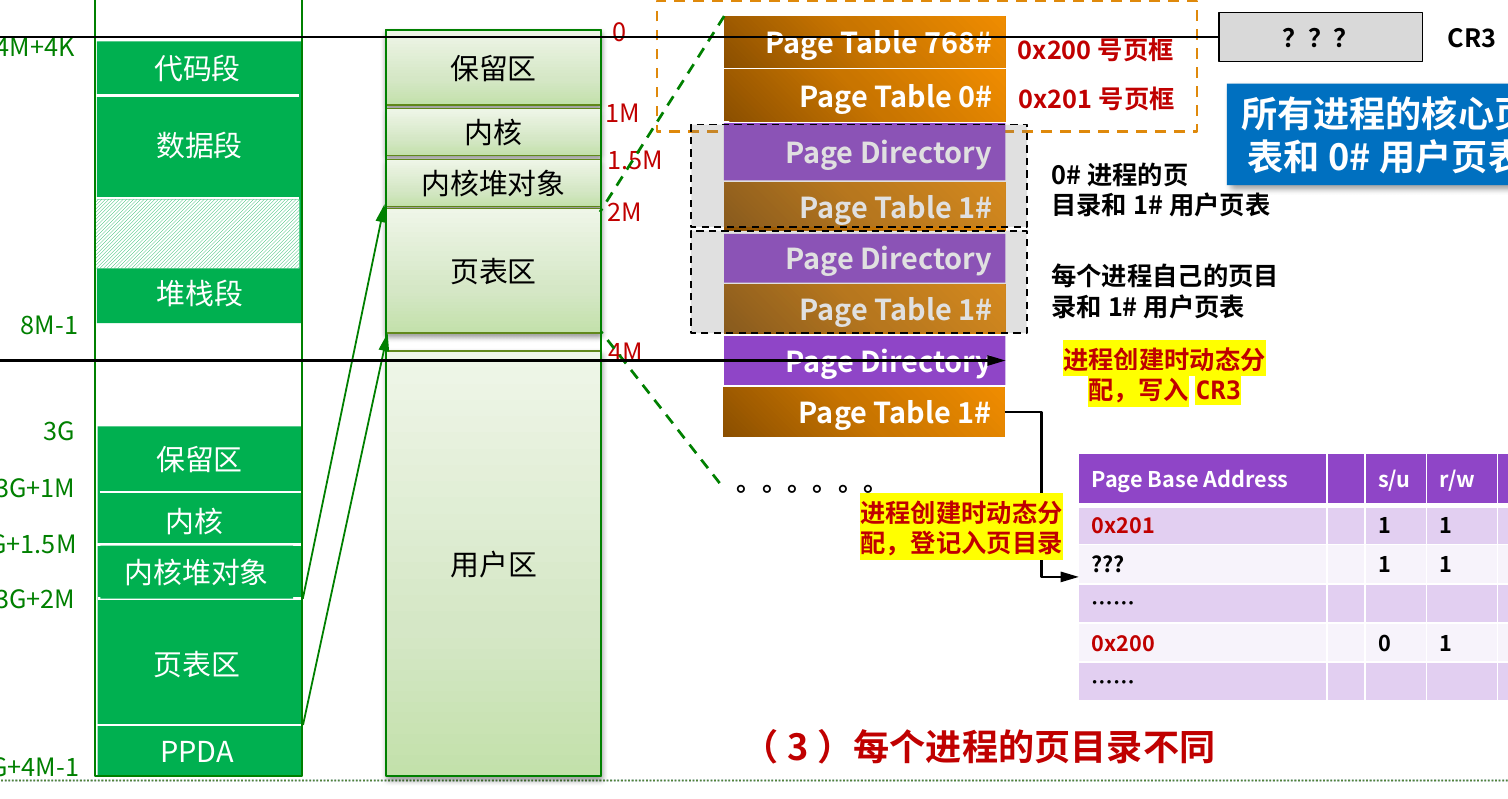
\includegraphics[width=0.85\textwidth]{figures/fig_private_pdir.png}
  \caption{每进程独立页目录与 CR3 的关系（图源：课程设计 PPT slide 10）}
  \label{fig:private-pdir}
\end{figure}

与每进程一张私有页目录相对应，\texttt{MemoryDescriptor} 也被简化为\textbf{只管理一页
私有用户页表}。\texttt{Initialize()} 只分配一页（而非原来的两张），
\texttt{Release()} 只回收一页，\texttt{ClearUserPageTable()} 只清除一页的表项。
这一变化是页表改造的直接结果：既然每进程只有一张私有用户页表（1\#），那么围绕它的
分配、回收与清零都自然以一页为单位。

\section{进程切换与 CR3 刷新}
页目录私有化之后，进程切换的核心动作就从"重写共享页表项"变成了"更换 \texttt{CR3}
指向目标进程的页目录"。这一变化集中体现在 \texttt{SwtchUStruct} 宏中：

\begin{lstlisting}[caption={进程切换宏 SwtchUStruct 的改造},label={lst:swtch}]
// 对应源码 (PPT slide 17)
#define SwtchUStruct(p)                                                         \
    Machine::Instance().GetKernelPageTable()                                    \
        .m_Entrys[Kernel::USER_PAGE_INDEX].m_PageBaseAddress = (p)->p_addr >> 12; \
    FlushPageDirectory((p)->GetPageDirectoryPhyAddr());
\end{lstlisting}

\begin{figure}[H]
  \centering
  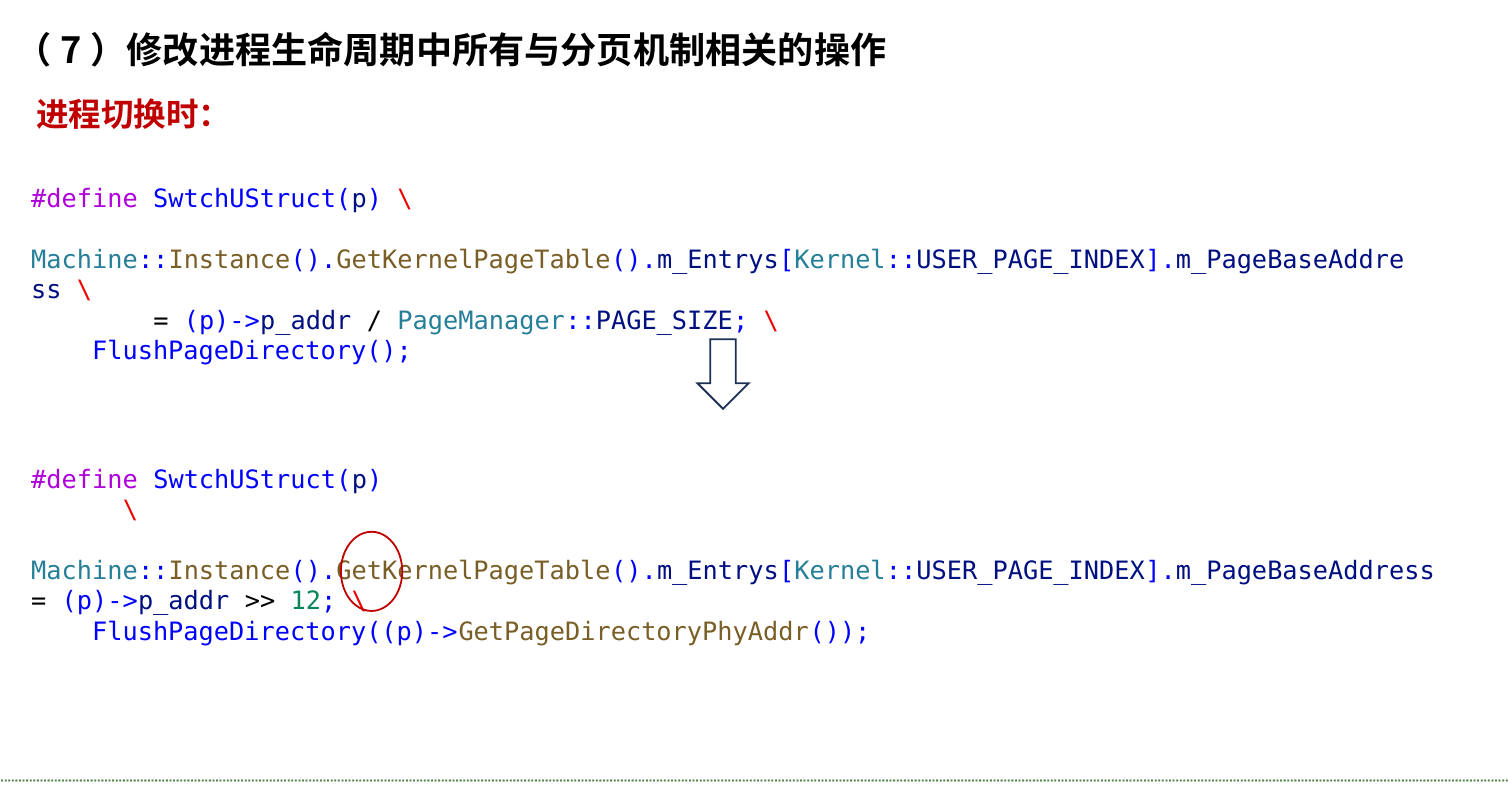
\includegraphics[width=0.85\textwidth]{figures/fig_swtch.png}
  \caption{进程切换宏 SwtchUStruct 的改造对比（图源：课程设计 PPT slide 17）}
  \label{fig:swtch}
\end{figure}

该宏完成两件事：其一，把核心页表中用于映射当前进程 user 结构（即 PPDA）的那一项，
更新为目标进程的 \texttt{p\_addr}（\texttt{Kernel::USER\_PAGE\_INDEX} 标识该 PTE 在
核心页表中的位置）；其二，调用 \texttt{FlushPageDirectory()} 把目标进程页目录的
物理地址写入 \texttt{CR3}，使新页目录立即生效。\texttt{FlushPageDirectory} 的实现
就是一条 \texttt{movl \%0, \%cr3} 指令。值得注意的是，与原系统固定刷新到
\texttt{0x200000} 不同，改造后的版本以目标进程的页目录物理地址为参数，这正是
"每进程独立页目录"在切换路径上的体现。

在进程管理器的 \texttt{Swtch()} 调度流程中，选中目标进程后还会调用
\texttt{MapToPageTable()}，其改造后实现同样只是调用
\texttt{FlushPageDirectory(u.u\_procp->GetPageDirectoryPhyAddr())}，确保当前
\texttt{CR3} 与 user 结构中记录的进程页目录保持一致。

\section{页表改造后的效果与边界}
经过上述改造，页表系统具备了如下能力：每个进程拥有独立的 4MB 用户空间映射
（由私有 1\# 用户页表决定），进程间地址空间相互隔离；进程切换不再重写页表项，
而是通过一次 \texttt{CR3} 写入完成；核心页表与 0\# 用户页表全局共享，避免了
冗余的初始化与切换开销。

同时也需明确改造的边界。\texttt{m\_UserPageTableArray} 仅指向一页私有用户页表，
因此凡涉及它的分配、回收、清除操作都以一页为单位——这与原系统两张用户页表的
做法不同，是页表布局变化带来的连带修改。此外，原系统中那些"与相对映射表设置物理
页表相关"的接口函数（如旧的 \texttt{MapEntry} 系列重载）在新模型下不再需要，
本次改造中已将其注释移除。这些边界修改为后续章节的位示图分配与进程映像管理奠定
了地址映射层面的基础。

\subsection*{运行验证}
页表系统改造完成后，内核能够正常引导启动并进入 shell。图~\ref{fig:run-shell-ch3}
为系统在 QEMU 下启动后进入 shell 提示符 \texttt{[/]\#}、并执行目录列出的画面，根
目录下可见 \texttt{dev}、\texttt{Shell.exe}、\texttt{etc}、\texttt{bin} 等条目。系统
能够启动并支撑 shell 运行，从运行层面验证了每进程独立页目录、核心页表恒等映射与
页目录初始化的正确性。

\begin{figure}[H]
  \centering
  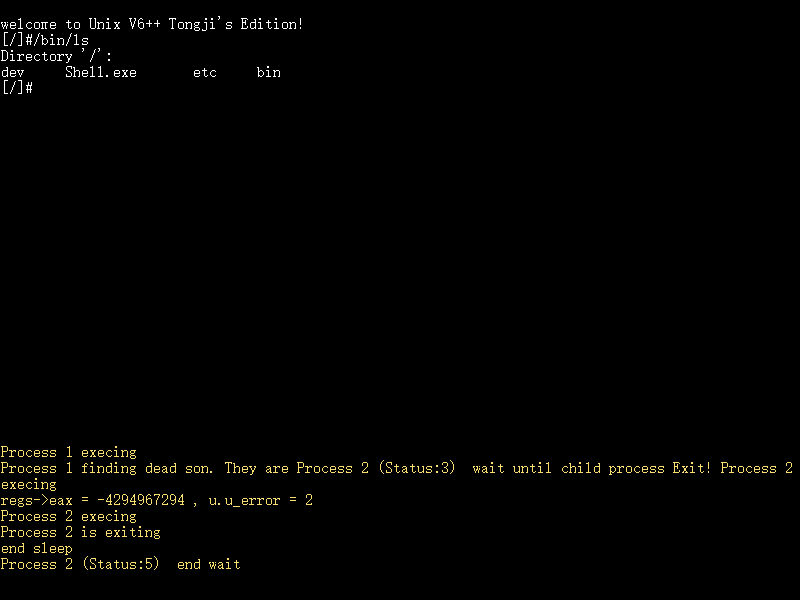
\includegraphics[width=0.85\textwidth]{figures/run_shell.png}
  \caption{页表系统改造后系统引导进入 shell}
  \label{fig:run-shell-ch3}
\end{figure}
